% Source: Code/ML_overlay/ir_rgb_registration/paper/ml_overlay_report_materials/ir_rgb_registration_report/figures/fig_accuracy_vs_speed_scatter.tex
\documentclass[tikz,border=10pt]{standalone}
\usepackage{pgfplots}
\usepackage{amssymb}
\pgfplotsset{compat=1.18}

\definecolor{Garnet}{RGB}{115,0,10}
\definecolor{Rose}{RGB}{204,46,64}
\definecolor{Atlantic}{RGB}{70,106,159}
\definecolor{Congaree}{RGB}{31,65,77}
\definecolor{Horseshoe}{RGB}{101,120,11}
\definecolor{Honeycomb}{RGB}{164,145,55}
\definecolor{Black90}{RGB}{54,54,54}
\definecolor{Black50}{RGB}{162,162,162}

\begin{document}
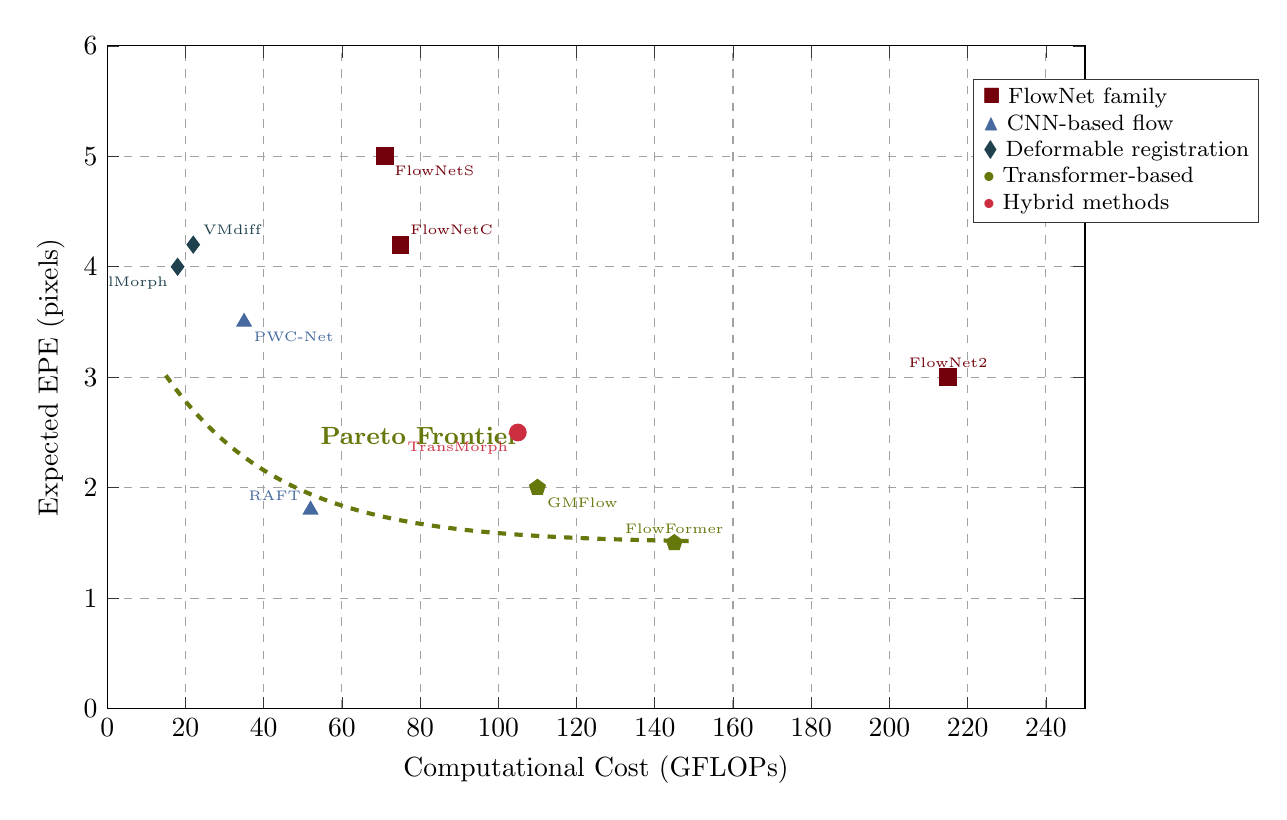
\begin{tikzpicture}
\begin{axis}[
    width=14cm,
    height=10cm,
    xlabel={Computational Cost (GFLOPs)},
    ylabel={Expected EPE (pixels)},
    xmin=0, xmax=250,
    ymin=0, ymax=6,
    grid=major,
    grid style={dashed,Black50},
    legend pos=north east,
    legend style={draw=Black90,fill=white,font=\footnotesize},
    tick style={Black90},
    scatter/classes={
        a={mark=square*,Garnet},
        b={mark=triangle*,Atlantic},
        c={mark=*,Congaree},
        d={mark=diamond*,Horseshoe},
        e={mark=pentagon*,Rose}
    }
]

% Pareto frontier annotation (approximate curve through best trade-offs)
\addplot[Horseshoe,dashed,line width=1.5pt,domain=15:150,samples=100] {1.5 + 2.5*exp(-x/30)};
\node[Horseshoe,font=\small\bfseries,anchor=south] at (axis cs:80,2.3) {Pareto Frontier};

% FlowNetS
\addplot[only marks,mark=square*,mark size=3pt,Garnet] coordinates {(71,5.0)};
\node[font=\tiny,Garnet,below right] at (axis cs:71,5.0) {FlowNetS};

% FlowNetC
\addplot[only marks,mark=square*,mark size=3pt,Garnet] coordinates {(75,4.2)};
\node[font=\tiny,Garnet,above right] at (axis cs:75,4.2) {FlowNetC};

% FlowNet2
\addplot[only marks,mark=square*,mark size=3pt,Garnet] coordinates {(215,3.0)};
\node[font=\tiny,Garnet,above] at (axis cs:215,3.0) {FlowNet2};

% PWC-Net
\addplot[only marks,mark=triangle*,mark size=3pt,Atlantic] coordinates {(35,3.5)};
\node[font=\tiny,Atlantic,below right] at (axis cs:35,3.5) {PWC-Net};

% RAFT
\addplot[only marks,mark=triangle*,mark size=3pt,Atlantic] coordinates {(52,1.8)};
\node[font=\tiny,Atlantic,above left] at (axis cs:52,1.8) {RAFT};

% VoxelMorph
\addplot[only marks,mark=diamond*,mark size=3pt,Congaree] coordinates {(18,4.0)};
\node[font=\tiny,Congaree,below left] at (axis cs:18,4.0) {VoxelMorph};

% VMdiff
\addplot[only marks,mark=diamond*,mark size=3pt,Congaree] coordinates {(22,4.2)};
\node[font=\tiny,Congaree,above right] at (axis cs:22,4.2) {VMdiff};

% GMFlow
\addplot[only marks,mark=pentagon*,mark size=3pt,Horseshoe] coordinates {(110,2.0)};
\node[font=\tiny,Horseshoe,below right] at (axis cs:110,2.0) {GMFlow};

% FlowFormer
\addplot[only marks,mark=pentagon*,mark size=3pt,Horseshoe] coordinates {(145,1.5)};
\node[font=\tiny,Horseshoe,above] at (axis cs:145,1.5) {FlowFormer};

% TransMorph
\addplot[only marks,mark=*,mark size=3pt,Rose] coordinates {(105,2.5)};
\node[font=\tiny,Rose,below left] at (axis cs:105,2.5) {TransMorph};

\end{axis}

% Legend outside plot
\node[draw=Black90,fill=white,font=\footnotesize,align=left,anchor=north west] at (11,8) {
    \textcolor{Garnet}{$\blacksquare$} FlowNet family\\
    \textcolor{Atlantic}{$\blacktriangle$} CNN-based flow\\
    \textcolor{Congaree}{$\blacklozenge$} Deformable registration\\
    \textcolor{Horseshoe}{$\bullet$} Transformer-based\\
    \textcolor{Rose}{$\bullet$} Hybrid methods
};

\end{tikzpicture}
\end{document}
